\chapter{Ergebnisse}

\section{Python-Interface f"ur MCTDH}
\label{sec:PyInterface}


Es wurden eine Programmierschnittstelle (englisch \textit{application programming interface}, API) f"ur das MCTDH-Programmpaket erstellt.
Im Rahmen dieser Arbeit wurde sich auf Klassen beschr"ankt, welche f"ur das Einlesen der baumf"ormig strukturierten MCTDH-Basis zust"andig sind.
Die Klassen und Methoden, die "uber Python aufgerufen werden k"onnen, sind in Abbildung \ref{fig:uml_Cython} dargestellt. 
Jede Klasse der API wird in Abbildung \ref{fig:uml_Cython} durch einen Kasten repr"asentiert. Im oberen Teil des Kastens ist der Klassenname
angegeben und im unteren Teil sind die Methoden der Klasse aufgelistet. 
\textit{ControlParameter} und \textit{mctdhBasis} sind die Klassen, die die Konfigurations- und Basisdatei einlesen. 
In der Klasse \textit{mctdhBasis} kann die Anzahl der Knoten des MCTDH-Baums aus dem Basisdatei ausgegeben werden.
Knoteneigenschaften k"onnen "uber die Klasse \textit{mctdhNode}  ermittelt werden. Dabei stellt ein Objekte dieser Klasse
eine Knoten dar.
So kann festgestellt werden, ob ein Knoten den obersten Knoten darstellt oder zu den untersten Knoten geh"ohrt und mit wieviel weiteren Knoten er verbunden ist.
Die Knotenobjekte k"onnen in Nachbarknoten "uberf"uhrt werden.
Die SPFs eines Knoten wird in der Klasse \textit{Tdim} ermittelt. Die  in die Klassen \textit{physCoor}. Mit diesen Klassen k"onnen
die Schwingungsmoden, der untersten Knoten, sowie die SPFs der jeweiligen Knoten ermittelt werden. 

\begin{figure}
    \centering
    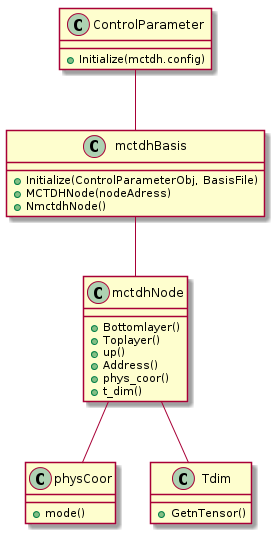
\includegraphics[scale=0.6]{figures/sequenceDiagram}
    \caption{Alle Klassen, die in Cython erstellt wurden, sind mit einem ,,C'' gekennzeichnet. Die jeweiligen Klassenmethoden sind mit einem
    gr"unen Punkt gekennzeichnet.}\label{fig:uml_Cython}
\end{figure}
Die in Abbildung \ref{fig:uml_Cython} k"onnen mit folgenden Befehl in Python aufgerufen werden:

\begin{verbatim}
import mctdh
\end{verbatim}

Um in Python die MCTDH-Klassen verwenden zu k"onnen, gen"ugt es \textit{mctdh} dem Klassennamen voranzustellen und durch eine Punkt zu trennen.

\begin{verbatim}
config = mctdh.controlParameters()
basis = mctdh.MctdhBasis()
\end{verbatim}

"Uber die initialisierten Objekte kann auf die Klassenmethoden zugegriffen werden: 
\begin{verbatim}
config.initialize('mctdh.config')
basis.initialize('basis.txt', config)
\end{verbatim}

Mithilfe des Objektes \textit{basis} k"onnen weitere Objekte anderer Klassen generiert werden.
In den folgenden Python-Funktionen werden Objekte der Klasse \textit{MctdhNode(), PhysCoor()} und \textit{Tdim()} erzeugt. 

\begin{verbatim}
    def getBottomlayer():
        bottom_list = []
        for i in range(basis.NmctdhNodes()):
            node = basis.MCTDHnode(i)
            if node.Bottomlayer() == True:
                bottom_list.append(i)
        return bottom_list
    
    def getPhysCoord():
        mode_list = []
        for i in range(basis.NmctdhNodes()):
            node = basis.MCTDHnode(i)
            if node.Bottomlayer() == True:
                phys = node.phys_coor()
                mode_list.append(phys.mode()) 
        return mode_list
    
    def get_SPFs():
        nodes_spf = {}
        for i in range(basis.NmctdhNodes()):
            node = basis.MCTDHnode(i)
            tdim = node.t_dim()
            nodes_spf[i] = tdim.GetnTensor() 
        return nodes_spf
\end{verbatim}

In der ersten Funktion wird eine Liste zur"uckgegeben, die die unteresten Knoten des eingelesenen MCTDH-Baums enth"alt.
Dabei werden die Methoden \textit{NmctdhNodes()} und \textit{Bottomlayer()} verwendet, um die Anzahle sowie die Lage der Knoten
ermitteln zu k"onnen. \textit{Bottomlayer()} ist eine Methode von \textit{MctdhNode()}.
In der zweiten Funktion wird eine Liste der Moden des MCTDH-Baums mithilfe der Methode \textit{mode()} von \textit{PhysCoor()} zur"uckgegeben. 
Und die letzte Funktion generiert eine Liste aus SPFs, die mithilfe der Methode \textit{GetnTensor()} von \textit{Tdim()}.
Die Objekte \textit{node, phys} und \textit{tdim} h"atten auch durch 

\begin{verbatim}
node = mctdh.MctdhNode()
phys = mctdh.PhysCoor()
tdim = mctdh.Tdim()
\end{verbatim}

initialisiert werden k"onnen. 
    

\section{Graphische Benutzeroberfl"ache f"ur MCTDH}

 Die graphisch Benutzeroberfl"ache (GUI) f"ur MCTDH-Rechnungen wurde in Python und Qt implementiert.
 Der Zugriff auf die Qt-Bibliothek erfolgt "uber die Python-Bibliothek PyQt4. 
 PyQt4 umfasst zehn Python-Module, die zusammen ungef"ahr 400 Klassen und 6000 Methoden und Funktionen enthalten. \cite{PyQt}

 \begin{figure}
    \centering
    \vspace*{-0.5cm}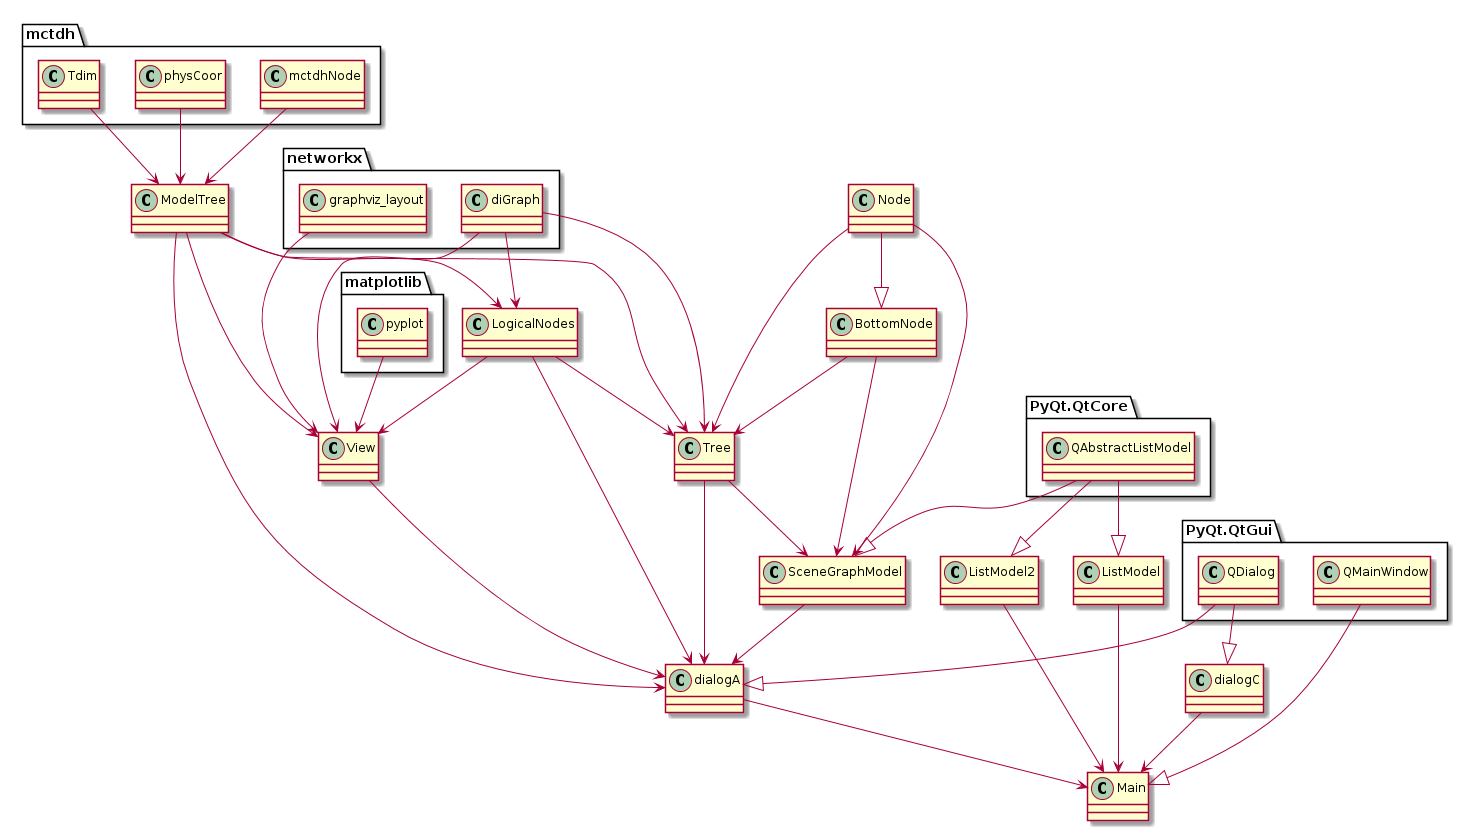
\includegraphics[width=\textwidth, angle=90, scale=1.4]{figures/umlPyQt}
    \caption{Klassendiagram der MCTDH-GUI. Eine Beschreibung des Diagramms
     findet sich im Text wieder.}\label{fig:uml_PyQt}
\end{figure}

In Abbildung \ref{fig:uml_PyQt} sind die wichtigen Klasse aufgef"uhrt, die f"ur die Implementierung der GUI verwendet wurden. 
Die Klassen, die in Rechtecken zusammengefasst wurden, entstammen aus Python-Modulen, deren Namen links "uber den Rechtecken angegeben sind.
Bei den Modulen handelt es sich um die PyQt4-Module \textit{QtCore} und \textit{QtGui}. F"ur die graphisch Darstellung der MCTDH-Baumdiagramme
wurden die Module \textit{matplotlib} und \textit{networkx} verwendet. Die Klassen, die in Abschnitt \ref{sec:PyInterface} vorgestellt wurden,
sind im Modul \textit{mctdh} enthalten. 

Alle \textit{mctdh}-Klassen werden in ModelTree verwendet, um alle Informationen zum MCTDH-Baum zu erhalten. Die Information wird an die
Klasse \textit{LogicalNodes} "ubergeben und es werden in dem Datentyp \textit{Dictionary} die Knoten des Baums mit den SPFs und f"ur den 
untersten Layers mit den Moden gespeichert. Speziell f"ur die Visualisierung von Baumdiagramme existiert das Python-Modul \textit{networkx}, 
aus dem die Klasse \textit{diGraph} verwendet wird, in der die Knoten gespeichert werden. Das Baumdiagramm wird in der Klasse \textit{View}
in einem \textit{png}-File mithilfe des Moduls \textit{matplotlib} gespeichert, das f"ur die Erzeugung von Diagrammen entwickelt wurde.
Das \textit{png}-File wird anschlie"send in der GUI verwendet. Die Informationen "uber den MCTDH-Baum wird von \textit{LogicalNodes}
auch an die Klasse \textit{Tree} "ubergeben.

Die Pfeile mit den ausgef"ullten Pfeilk"opfen  f"uhren von Klassen, die in anderen Klassen verwendet werden,
auf die die Pfeilspitze zeigt. 
Auf die Klassen, die durch Vererbung erstellt wurden, zeigen rot umrandete Pfeilspitzen. Beispielswei"se f"uhren diese Pfeile von allen angegeben PyQt-Klassen
, von denen geerbt wird.
Sowohl von \textit{QDialog} als auch \textit{QMainWindow} werden durch Vererbung Unterklassen generiert: \textit{dialogA, dialogc} und \textit{Main}. 
Allerdings wurden diese drei Klassen in Qt-Designer erzeugt, in dem die jeweiligen Fenster mit den ben"otigten Steuerungselementen zusammengestellt werden 
k"onnen. So k"onnen die Gr"o"sen der Steuerungselemente ohne Programmierung per Maus festgelegt werden. Die Informationen "uber 
die jeweiligen Fenster werden in \textit{ui}-Dateien gespeichert. Mit PyQt k"onnen diese Dateien eingelesen werden und aus den Daten die entsprechenden 
Klassen erstellt und beliebig erweitert werden.
Die beiden Klassen\textit{QDialog} und \textit{QMainWindow} stammen von \textit{QWidget} ab. \textit{QWidget}, \textit{QDialog} und \textit{QMainWindow}
sind Steuerungselement, mit denen der Benutzer durch die Tastatur und Maus interagieren kann. \cite{PyQt}

Die Klasse \textit{Main} stellt das Hauptfenster der GUI dar, von dem aus neue Projektordner erstellt, umbenannt oder gel"oscht werden k"onnen.
In diesen Ordner finden sich wiederum Ordner, die Einstellungen unterschiedlicher Rechnungen enthalten. Schlie"slich k"onnen aus
dem Hauptfenster neben der Ordernderverwaltung MCT\-DH-Rechnungen gestartet werden.
Die Klasse \textit{dialogC} generiert eine Fenster, in dem die Ordnernamen eingetragen werden k"onnen, um entweder neue Ordner zu erstellen
oder alte Ordner um zu benennen.
Die Einstellungsparameter einer MCTDH-Rechnung werden in der Klasse \textit{dialogA} angegeben. Bereits existierende MCTDH-Basisfiles werden
eingelesen und im \textit{dialogA}-Fenster dargestellt.


Alle Steuerungselement wie Kn"opfe, Checkboxen oder Elemente innerhalb eines Fensters emittieren Signale aus, die Aktionen des Benutzers
zugeordnet werden k"onnen. Aktionen k"onnen das Einmal- oder Doppeltklicken, das Bewegen des Mauszeigers oder das Bet"attigen der Entertaste sein.
Einzelne Steuerungselemente k"onnen zusammen mit einer bestimmten Aktion mit einer Klassenmethode bzw. Funktion verbunden werden, die die Klassenmethoden ausl"osen. 
  

Qt enth"alt Klassen, mit denen beliebig viele Elemente dargestellt werden k"onnen. Diesen Klassen liegt eine Model/View-Aufbau zugrunde,
 der das Datenmodel von der Darstellung der Daten trennt. 
Ein Datenmodel ist die Klasse \textit{QAbstractListModel}, in die die Daten eingelesen, bearbeitet und gel"oscht werden k"onnen.
Die Daten k"onnen wiederum in den Klassen \textit{QListView} und \textit{QTreeView} dargestellt werden. 
Die Trennung zwischen dem Datenmodel und der graphischen Darstellung der Daten beruht auf dem Model-View-Controller (MVC) Paradigma.\cite{Qt}  

Bei der MVC-Programmierung werden verschiedener Klassen erstellt. Jede dieser Klassen erf"ullt unterschiedliche Aufgaben:
die Verarbeitung von Daten innerhalb der
Anwendungssoftware (Model), die Visualisierung des aktuellen Systemzustandes (View) und die Interaktion zwischen Benutzer und Programm (Controller). \cite{MVC}

In Qt wurden der Controller und View kombiniert, sodass die Speicherung und Bearbeitung der Daten  von der Datenvisualisierung  
getrennt wurde. Die gleichen Daten k"onnen in verschieden Ansichten dargestellt werden. 
Die Implementierung neuer Darstellungsarten "andert nicht die darunterliegende Datenstruktur.\cite{Qt} 
Der Vorteil der Model/View-Architektur ist, dass die Element, die die visualisierten Daten des Models darstellen, nicht jeweils mit einer
Funktion gekoppelt werden muss wie bei anderen Steuerungselementen. So k"onnen Aktionen beliebig vieler Elemente 
mit nur einer Funktion verbunden werden. Dabei wird nur das Steuerungselement, das die Daten darstellt, mit den gew"unschten
Aktionen verbunden, wobei Aktionen auf ein beliebiges Element innerhalb der Steuerungselemente Informationen "uber dieses Element 
in Bezug auf das Datenmodel an die Funktion "ubertr"agt.

Qt besitzt f"ur die Model/View-Architektur Standardmodel, allerdings k"onnen die Modelle durch die Vererbung
von QAbstractListModel ver"andert und angepasst werden. So bekommt \textit{SceneGraphModel} keine Liste als Eingabetype wie die Klassen \textit{ListModel} und
\textit{ListModel2},
sondern Objekte der Klassen \textit{Node} und \textit{BottomNode}. 
Die Klasse \textit{BottomNode} erbt von \textit{Node} und enth"alt zus"atzlich Informationen zu den Moden der untersten Knoten. 
\textit{Node}-Objekte spiegeln bestimmte Knoten des
MCTDH-Baums wieder, in denen Informationen zu Elternknoten und Kinderknoten gespeichert sind. Diese Objekte werden
in der Klasse \textit{Tree} in einem \textit{Dictionary} zum Baum zusammengefasst. 
Die Daten des Models aus \textit{SceneGraphModel} werden "uber die PyQt-Klasse QTreeView in \textit{dialogA} visualisiert.
\textit{ListModel} und \textit{ListModel2} enth"alt eine Liste der Projektordner und der Ordner verschiedener Rechnungen innerhalb der Projekte.
Diese Daten werden in zwei getrennten QListView dargestellt und k"onnen mithilfe des Models aktualisiert werden.




  




   
